\chapter{Estado del Arte}

En este capítulo hablaremos, principalmente, sobre dos importantes aspectos. El primero es la situación de la industria del entretenimiento digital hoy en día y qué es un \textit{roguelike}. El segundo son los elementos que dificultan y facilitan el uso de diferentes programas y \textit{software} a ciertos sectores de la sociedad como invidentes o daltónicos, cómo algunso programas intentan solventar estos problemas, qué opciones de accesibilidad existen en diferentes sistemas operativos y las razones por las que hemos elegido ciertas de las características de las que hemos dotado a nuestro proyecto.

\section{La industria del entretenimiento digital en la actualidad}

Desde sus primeros pasos hasta hoy en día, tal y como sucede con muchas de las novedades en el mundo del entretenimiento y la cultura, el sector del ocio digital ha sufrido cierto estigma por una gran parte de la población, siendo censurado y degragado en mayor o menor medida, no tan solo por cierta parte de la sociedad, pero también por muchos medios de comunicación y gobiernos. A pesar de que hoy en día este problema todavía está activo\footnote{Es común que cada año en Australia se censuren algunos juegos como \href{http://goo.gl/hFrQah}{Paranautical Activity} por razones que otras formas de entretenimiento y cultura como películas o libros no se ven tan afectados.}, la industria se ha expandido tanto (consolas, ordenadores, navegadores, Facebook, móvil...), que cada vez es más complicado encontrar a alguien que no haya jugado a algún videojuego en las últimas semanas y ya es algo que forma parte del día a día de mucha parte de la población.

\subsection{La industria, en números}
En todo el mundo, pero especialmente en EEUU, la industria de los videojuegos es uno de los sectores con más crecimiento\footnote{\url{http://www.theesa.com/wp-content/uploads/2014/11/Games_Economy-11-4-14.pdf}} llegando a generar, solamente en ventas digitales, alrededor de 61 billones de dólares en el año 2015\footnote{http://goo.gl/BgGhXy}.

Este gran éxito se debe, en gran parte, a la irrupción de los juegos desarrollados para móviles, cuyo beneficio ha ido aumentando enormemente durante los últimos años. \footnote{\href{http://goo.gl/Lz9UAa}{La venta de videojuegos en Alemania crece año tras año, pero el mayor aumento de beneficio se está centrando en el mercado de los juegos para móvil}}. Sin embargo, esto no significa que el resto de plataformas no estén triunfando. Solamente Steam, la plataforma de distribución digital para PC por excelencia desarrollada por Valve, ha generado alrededor de 3 billones y medio de dólares en el año 2015\footnote{\url{http://goo.gl/Mbjgol}}.

Con el mercado del PC resurgiendo, las consolas de sobremesa obteniendo grandes números de ventas, las portátiles resistiendo, el mercado de los videojuegos para móvil en esplendor y los cascos de realidad virtual llegando al mercado este año 2016; todo parece indicar que estos números no harán más que crecer en los próximos años.

\subsection{Conclusión}

Lo que comenzó hace varias décadas como un modo de entretenimiento sin ninguna pretensión, generalmente enfocado a adolescentes y que miraba a otras industrias como la cinematográfica con recelo, se ha convertido en todo lo que había deseado y más. Gracias a grandes títulos y a su expansión a toda clase de dispositivos, no se puede hablar de la industria del entretenimiento sin hablar de videojuegos y en muchos casos algunos de esos títulos han logrado ser nombrados como obras de arte en su género, pasando a la historia y siendo recordados a lo largo de los años.

Sin embargo, es bastante probable que lo mejor esté todavía por llegar.

\section{\textit{Roguelikes.}}

\subsection{Qué es y orígenes}

En 1983, Michael Toy y Glenn Wichman crearon un videojuego llamado Rogue\footnote{Desde 2014 este juego se encuentra disponible en \href{https://archive.org/details/msdos_Rogue_1983}{archive.org}} que acabó definiendo un género.

Las características principales que definieron a Rogue y que, por extensión, definieron al género de los \textit{roguelikes} inicialmente, son:

\paragraph{Dificultad}: Rogue es un videojuego difícil con \textit{permadeath}\footnote{Una vez que el jugador muere, tiene que empezar desde el principio; no hay partidas guardadas} que obligará al jugador a rejugarlo una y otra vez, intentando llegar más lejos que la anterior partida gracias a ir aprendiendo los funcionamientos del mismo.

\paragraph{Aleatoriedad}: Cada vez que el jugador comienza una partida nueva se encontrará con ciertos elementos que han cambiado con respecto a la anterior: el mapa es diferente, los elementos y enemigos se encuentran en sitios distintios, los propios objetos han cambiado... causando que cada vez que el usuario empiece, tenga un grado de dificultad pseudo-aleatorio dependiendo de la semilla con la que estos elementos han sido generados.

\paragraph{Progresión}: Una de las frases más escuchadas en las críticas que Rogue recibió tras su lanzamiento es que el jugador sentía la necesidad de intentar llegar más lejos en cada ocasión\footnote{Jerry Pournelle habló de ello en \href{http://goo.gl/Iz2qg6}{este artículo}}. Esto viene dado, sobre todo, por la sensación de progresión y de que en cada \textit{run}\footnote{Palabra comúnmente usada en estos géneros y que se refiere a una partida desde su inicio hasta que el jugador pierde} el usuario va mejorando.

\begin{figure}[h!]
		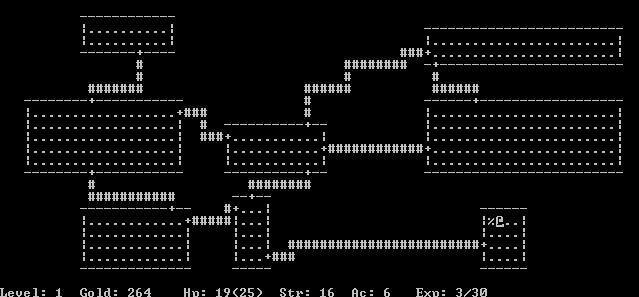
\includegraphics[width=\textwidth,height=\textheight,keepaspectratio]{./img/roguegame.PNG}
	\caption{Captura de pantalla de \href{https://en.wikipedia.org/wiki/File:Rogue_Unix_Screenshot_CAR.PNG}{dominio público} (tal y como todas las imágenes mostradas en este proyecto) del videojuego Rogue}
	\label{fig:roguegame}
\end{figure}

A partir de este momento muchos fueron los juegos que decidieron imitar estas características de Rogue, solamente cambiando diferentes elementos, por eso se han denominado \textit{roguelikes}.

\subsection{En la actualidad}

Tras el éxito de Rogue, fueron muchos los títulos que simularon su fórmula de éxito e intentaron mejorarlo, sobre todo gráficamente. Muchos de ellos se centran en diferentes elementos (combate en vez de exploración, por ejemplo) y llegan a ser completamente diferentes a la hora de jugarlos (por turnos o tiempo real) pero, sin embargo, todos conservan buena parte de las características que hicieron al género famoso hasta hoy en día, al menos muchos de ellos.

\begin{figure}[h!]
		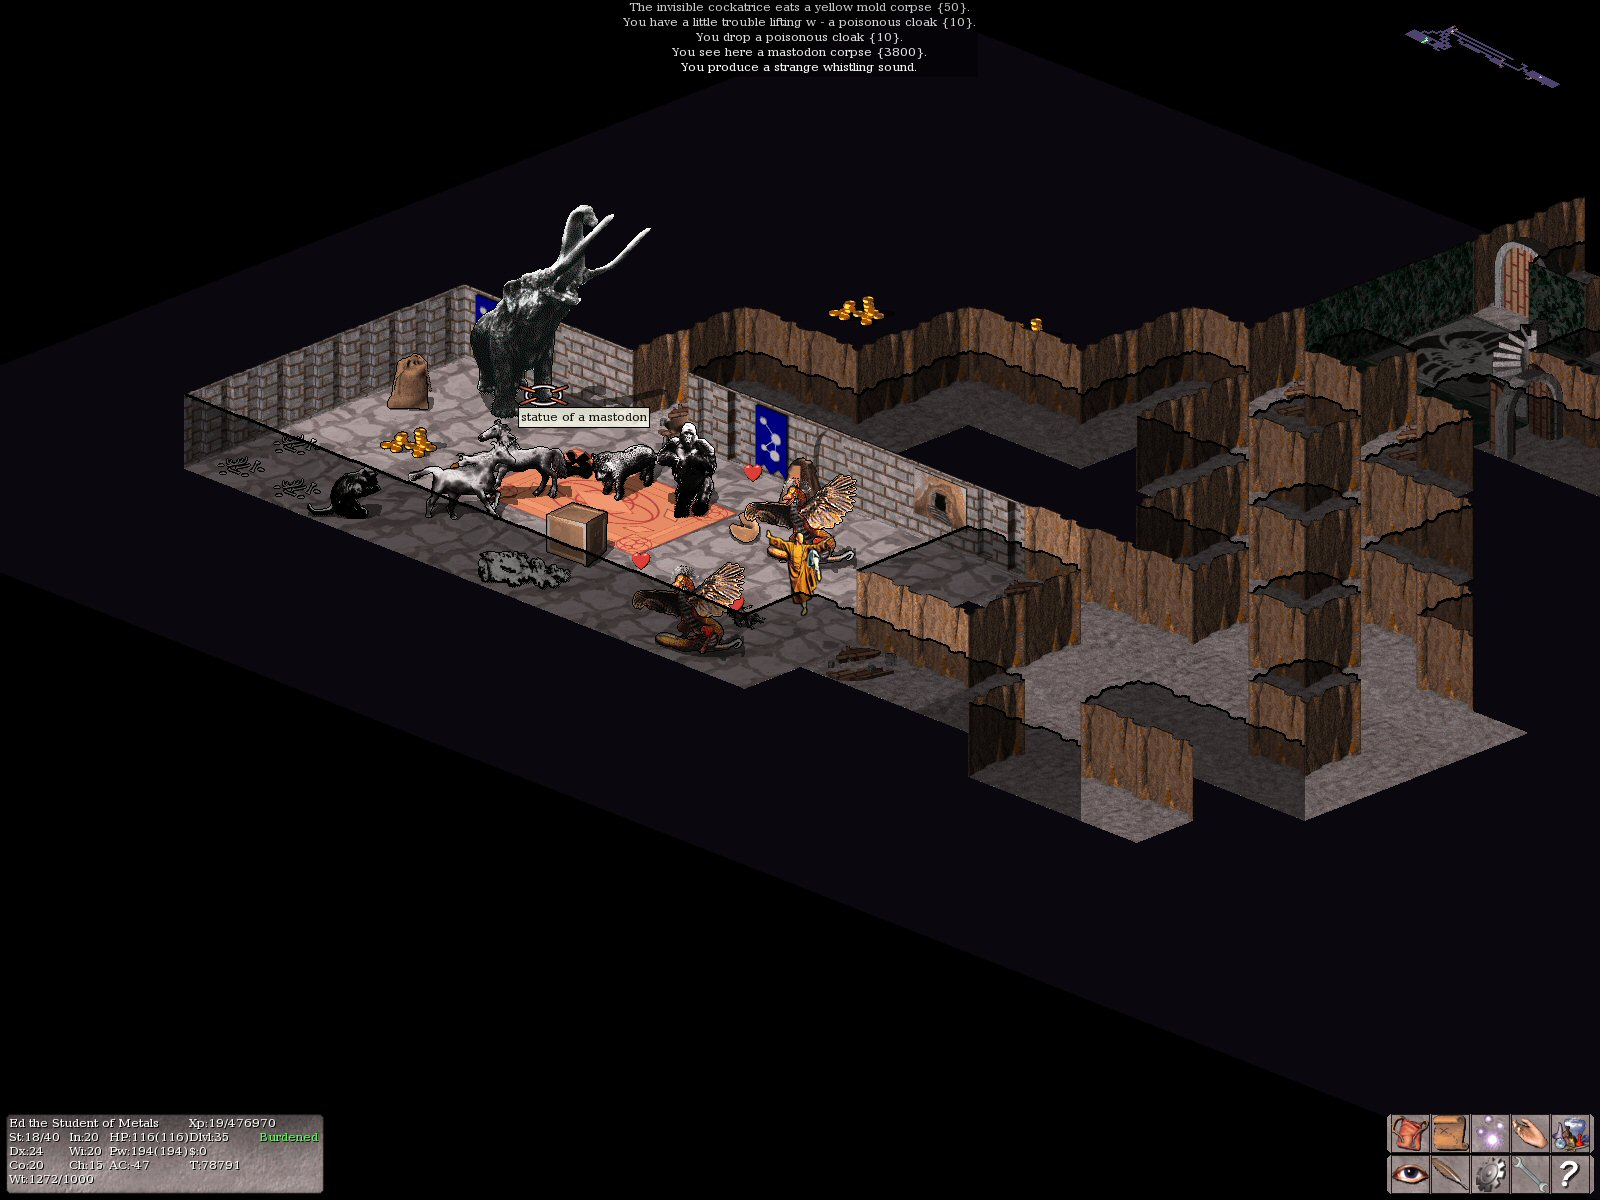
\includegraphics[width=\textwidth,height=\textheight,keepaspectratio]{./img/Vultures.jpg}
	\caption{Captura de pantalla del videojuego Vultures}
	\label{fig:vulturesgame}
\end{figure}

\subsubsection{La creación de subgéneros}

Dado que perder todo el progreso y tener que empezar desde el principio sin haber conseguido nada más que la experiencia personal es algo que no atrae a mucha gente hoy en día, son numerosos los juegos que han añadido más elementos de progreso general para que el jugador no se sienta frustrado. Estos elementos pueden ser nuevos personajes con los que jugar, puntos de experiencia o dinero con lo que poder equipar y mejorar desde un principio a nuestro personaje para poder llegar más lejos que la anterior vez.
También es común ver juegos que se basan en partidas cortas, de como mucho una hora, para que la repetición sea continua y parte de la experiencia en vez de un ``castigo'' que tener que afrontar.

Estos cambios que se han realizado durante los últimos años y que, de cierta manera, han modificado el género que Rogue creó en un inicio, no siempre se han tomado positivamente por parte de la comunidad, quejándose de que muchos títulos que se definen a sí mismos como \textit{roguelike} no contienen ciertos elementos, como la dificultad, que una vez definieron el género. Por este motivo se han definido subgéneros como el \textit{roguelite}, que toman muchas de esas características, pero añaden o ignoran otras muchas para crear un título que sea un poco más sencillo y no penalice tanto al jugador.

\subsection{Elementos \textit{roguelike} en nuestro proyecto}

En nuestro caso hemos creado un \textit{roguelike} similar a Rogue, no solamente estéticamente, pero también en diseño y funcionalidad. El usuario se moverá por un mapa aleatoriamente generado y luchará contra diferentes enemigos que intentarán eliminarlo de diferentes formas. 

El objectivo del juego es llegar lo más lejos posible dentro de la mazmorra. Cada vez que el jugador entra en un portal se añadirá un punto (el número de puntos se mostrará en la pantalla) y, cada vez que esto suceda, un nuevo mapa, con diferentes características y contenido, será generado. El juego es complicado, aleatorio y con una sensación de progreso, tal y como el género \textit{roguelike} especifica.

INTRODUCIR IMAGEN DE NUESTRO JUEGO